\chapter{Generalised Bayesian Inference with Sets of Priors}
\label{cha:gbi}

\begin{itemize}
\item Short introduction to IP (sets of priors, lower/upper prevision/probability)
%\item motivate imprecise priors with ress paper: \cite{Troffaes2013a} --- now in intro
\item \pdc\ (Evans \& Moshonov, Fuquene-Cook-Pericchi), examples (Festschrift paper: \cite{Walter2010a})
\item further motivations for IP (ITIP chapter \cite{itip-statinf}) 
\item Generalized Bayesian inference
\item Generalized Bayesian inference with sets of priors
 \begin{itemize}
 \item sets of priors, GBR, robust Bayes
 \item sets of conjugate priors in general
 \item parameter set shapes
 \end{itemize}
\item IDM
\item JSTP paper \cite{Walter2009a}
\item isipta11 paper \cite{Walter2011a}
\item boatshape?
\end{itemize}



After having seen a detailed example for Bayesian inference using sets of conjugate priors in Section~\ref{sec:commoncause},
in the main chapter of this thesis,
we will give now a general introduction to the methodology of Bayesian inference with sets of conjugate priors.
In Section~\ref{sec:ip-intro} below, we will try to outline the general theory of imprecise or interval probability,
describing its main formulations and interpretations.
Section~\ref{sec:motivation} then gives at first some general motives for the use of imprecise probability methodology,
concluding with the motives especially relevant in the context of the Bayesian approach to statistical inference.
Then, Section~\ref{sec:imprecisebayes-conjugate} ****
***Section~\ref{sec:alternatives} ****


\section{Imprecise or Interval Probability}
\label{sec:ip-intro}

This Section will give a condensed introduction to the main theoretic concepts
in interval or imprecise probability as needed for the topics discussed in this thesis.
Here, we take a decidedly epistemic view on interval or imprecise probability,
as we will argue in Section~\ref{sec:motivation} that often,
imprecise probability distributions are a better tool for expressing prior beliefs
than precise probability distributions.

%While Section~\ref{sec:ip-general} follows mostly \textcite{2011:IESS-ip},
%Section~\ref{sec:ip-main} is based mainly on \textcite{1996:walley::expert} and \textcite{2000:walley::towards}.


\subsection{General Concept and Basic Interpretation}
\label{sec:ip-general}

The central idea of imprecise or interval probability \parencite{1991:walley, 2001:weichselberger, 2011:IESS-ip} is
to replace the usual, precise probability measure $\p(A)$ for events $A$%
\footnote{Events of interest $A$ are taken to be subsets of the sample space $\Omega$,
forming a $\sigma$-algebra, a non-empty collection of sets including countable unions and intersections of subsets of $\Omega$.}
with a \emph{lower} and \emph{upper probability}, denoted by $\Pl(A)$ and $\Pu(A)$, respectively,
satisfying
\begin{equation}
\label{eq:0ip1}
0 \le \Pl(A) \le \Pu(A) \le 1\,.
\end{equation}
In this setting, a usual probability measure forms the extreme case $\Pl(A) = \Pu(A) = \p(A)$,
when there is enough information to determine the distribution on the sample space $\Omega$
in precise stochastic terms.
On the other extreme, when $\Pl(A) = 0$ and $\Pu(A) = 1$,
we have no information at all on the probability for $A$ to occur,
and intermediate cases $0 \le \Pl(A) < \Pu(A) \le 1$ represent
different degrees of knowledge on this probability.

Therefore, interval or imprecise probability adds another modeling dimension:
While usual, precise probability measures can be used to model phenomena when there is perfect stochastical information,
like, e.g., in a lottery where the number of winning tickets (and the total number of tickets) is precisely known,
imprecise probability measures can account for cases where there is uncertainty about the probabilities themselves,
just like in a lottery where the number of winning tickets is not exactly known.
Non-stochastic uncertainty about model features like probabilities is often called \emph{ambiguity},
forming a crucial part of the human decision process,
and there are studies suggesting that humans process ambiguity in a way
differing from pure probabilistic reasoning \parencite{2005:hsu-bhatt}.

In contrast to a probability measure $\p(A)$,
the set functions $\Pl(A)$ and $\Pu(A)$ do not adhere
to the additivity axiom of Kolmogorov's \parencite*{1933:kolmogorov}
formalization of probability as a normed measure,
%(countable or finite additivity),
and thus are also known as \emph{non-additive probabilities}.
There is also a link to \emph{fuzzy measures}, which are also non-additive measures
\parencite[see, e.g.,][]{1997:denneberg}.

In general, $\Pl(A)$ may be understood as accounting for evidence certainly in favour of $A$,
and $\Pu(A)$ accounting for all evidence speaking not strictly against $A$.
The difference of $\Pu(A)$ and $\Pl(A)$ thus allows for inconclusive evidence
that may not speak unanimously in favor of or against $A$, respectively.
As evidence strictly against $A$ can be seen as evidence certainly in favour of $A^\com$,
the complement of $A$,
it is mostly assumed that $\Pl(A^\com) = 1 - \Pu(A)$,
and thus it suffices to determine either of $\Pl$ or $\Pu$,
the other one being defined through this relation.

There are currently two main approaches to a general theory of statistical inference with interval or imprecise probability:
\begin{enumerate}[(i)]
\item The theory by Weichselberger \parencite*{2000:weichselberger, 2001:weichselberger}
regards probability intervals $[\Pl(A), \Pu(A)]$ for all or some events $A$ as the basic entity
\parencite[p.~646]{2011:IESS-ip},
from which an interval-valued distribution on the sample space $\Omega$ is constructed.
His approach is axiomatic, in the sense that it replaces Kolmogorov's \parencite*{1933:kolmogorov} additivity axiom by two axioms,%
\footnote{The first states that \eqref{eq:0ip1} holds,
the second that the set $\mathcal{M}$ consisting of all usual, precise distributions $\p(\cdot)$
with $\Pl(A) \le \p(A) \le \Pu(A)$, for all $A \in \Omega$, is non-empty.
The second axiom guarantees that there exists at least one precise probability distribution
which is compatible with an interval-valued probability distribution,
and thus rules out the case of contradictory assignments of $[\Pl(A), \Pu(A)]$.}
from which the theory is derived,
while imposing no specific interpretation on these constructs.
This theory of interval probability was developed
as the foundation of a concept of \emph{logical probability} \parencite{2007:weichselberger},
where probability is not assigned to events, but to logical conclusions (from a premise to a consequence),
with the aim to arrive at a theory of statistical inference
which allows for fiducial-like probability statements,
e.g., probability statements on parameters similar to those derived from a posterior distribution in a Bayesian setting,
but without the need to specify a prior distribution \parencite[see, e.g.,][]{2011:IESS-fiducial}.
\item In contrast, the theory by Walley \parencite*{1991:walley, 2000:walley::towards}
aims to generalise the Bayesian approach to statistical inference,
adopting a strictly subjective, behavioural interpretation for imprecise probability
as lower and upper betting rates (see below),
and extending the Bayesian inference paradigm (as discussed in Section~\ref{sec:bayes-inference})
to imprecise probability distributions.
In generalising de Finetti \parencite*{1937:finetti,1970:finetti}, the basic entities are lower and upper \emph{previsions},
i.e.\ expectation functionals, for \emph{gambles}, i.e.\ random quantities,
instead of lower and upper probabilities for events.
This is due to the fact that unlike in the theory of precise probability%
---where the definition of a distribution via expectations %precise previsions
(often denoted \emph{linear previsions} in the imprecise probability literature)
is eqivalent to a definition via a precise probability distribution---%
the definition of an imprecise distribution via lower and upper previsions
is more general than a definition via lower and upper probability for events
\parencite[p.~132]{2000:walley::towards}.
\end{enumerate}
As this thesis is concerned with a generalization of Bayesian inference
based on sets of conjugate priors, the approach by Walley,
and its reliance on a subjective, epistemic interpretation of (imprecise) probability
as (bounds for) betting rates, is now described in more detail.


\subsection{Main Formulations}
\label{sec:ip-main}

%lower and upper probabilities or expectations,
%link to sets of probability distributions,
%sets of desirable gambles as mathematical formulation,
%lower and upper betting rates,
%inference procedure (itip)

The main mathematical formulations for imprecise distributions
in the theory by Walley \parencite*{1991:walley, 2000:walley::towards}
are
\begin{enumerate}[(i)]
\item lower previsions,
\item sets of (precise) probability distributions, and
\item sets of desirable gambles.
\end{enumerate}
It is possible to switch between these formulations,
although (ii) can be slightly more general than (i),
and to a greater extent, (iii) is more general than (ii) \parencite{2000:walley::towards}.

We will first introduce lower previsions
and the most important rationality requirements guiding their assessment and use,
then have a brief look at sets of desirable gambles as the most comprehensive formulation.
Sets of probability distributions, as the formulation used to describe inference models in this thesis,
are then explained in relation to the other formulations,
and the generalised Bayesian inference procedure as used in Section~\ref{sec:imprecise-alpha} is justified formally.

\subsubsection{Lower Previsions}

As mentioned in Section~\ref{sec:ip-general}, the basic entities in the theory by \textcite{1991:walley}
are lower and upper \emph{previsions}.
These are functions on \emph{gambles}, or \emph{random variables},
defined as bounded mappings from $\Omega$ to $\reals$.
A gamble $X$ can be understood as uncertain reward or payout,
where the reward $X(\omega)$ depends on $\omega \in \Omega$,
the unknown `state of the world' from the possibility space $\Omega$.
The reward is measured in units of utility assumed to form a linear scale
\parencite[\S 2.2]{1991:walley}.

A \emph{lower prevision} or \emph{lower expectation} is then a mapping
$\El: \mathcal{K} \to \reals$, where $\mathcal{K}$ is a set of gambles.%
\footnote{In Walley's central monography \parencite{1991:walley},
his papers and the imprecise probability literature in general,
lower previsions are usually denoted by $\Pl$.
There, an event $A \subset \Omega$ is notationally identified with the
indicator function $I_A(\omega)$, being a gamble with payout $1$ if $\omega \in A$ and else $0$,
such that $\Pl(A)$ denotes the lower probability of $A$.
In order to follow conventions in statistical literature, however,
lower previsions are denoted by $\El$ here,
and $\Pl$ refers to lower probabilities only.}
Central to Walley's theory is the interpretation of $\El[X]$
as the subject's supremum buying price for $X$, that is,
the subject is disposed to pay at most the fixed amount $\El[X]$
in exchange for the uncertain reward $X$.%
\footnote{More precisely, the price the subject is disposed to pay for $X$ is strictly less than $\El[X]$.
For sake of readability,
this mathematically important distinction is not rigorously maintained in this brief treatment,
as it is hardly relevant for the interpretation of the results in the later parts of this thesis.}
$\El[X]$ thus expresses the subject's state of knowledge about the value of $X$,
factoring in the propensity of all possible $\omega \in \Omega$
with their specific payouts $X(\omega)$.
The \emph{upper prevision} $\Eu[X]$ is the infimum selling price for $X$,
i.e., the fixed amount the subject is willing to receive in exchange for $X$
\parencite[p.~9]{1996:walley::expert}.
Walley's theory is based on this behavioral, epistemic interpretation of previsions,
%\parencite[Section~4]{1996:walley::expert},
and all rationality criteria and inference procedures
are deduced from this root \parencite[p.~5]{1996:walley::expert}.

The theory allows thus a zone of indeterminacy, by $\El[X] < \Eu[X]$,
for prices of $X$ at which the subject is neither willing to buy nor to sell the gamble $X$,
as illustrated in Figure~\ref{fig:pricesforgambles}.
This is in contrast to the usual epistemic operationalisation of subjective Bayesian probability,
which implies that $\El[X]$ and $\Eu[X]$ must coincide at a unique fair price $\E[X]$.
This requirement is refuted by Walley, and called by him \emph{the Bayesian dogma of precision}
\parencite[\S 5]{1991:walley}.

\begin{figure}
\centering
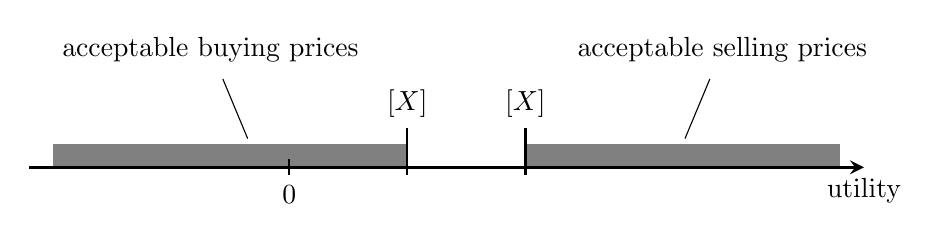
\begin{tikzpicture}[%
linkline/.style={
  shorten >= 2pt,
  shorten <= 3pt
}%
]
\path[fill=gray] (0,0) rectangle (4.5,0.3);
\path[fill=gray] (6,0) rectangle (10,0.3);
\draw[very thick,-stealth] (-0.3,0) -- (10.3,0) node[below] {utility};
\draw[thick] (3,0.1) -- (3,-0.1) node[below] {$0$};
\draw[thick] (4.5,-0.1) -- (4.5,0.5) node[above] {$\El[X]$};
\draw[thick] (6,-0.1) -- (6,0.5) node[above] {$\Eu[X]$};
\node (buy) at (2,1.5) {acceptable buying prices};
\node (sell) at (8.5,1.5) {acceptable selling prices};
\draw[linkline] (buy) -- (2.5,0.3);
\draw[linkline] (sell) -- (8,0.3);
\end{tikzpicture}
\caption{\label{fig:pricesforgambles}%
Illustration of \underline{E}\ and $\Eu$ as supremum buying and infimum selling prices for a gamble $X$ on a linear utility scale.}
%$\El$ %strange errors occur
\end{figure}

A lower and upper prevision are called \emph{conjugate}%
\footnote{Conjugacy in this sense should not be confused
with conjugacy for prior distributions as discussed in Section~\ref{sec:regularconjugates}.}
if the relation $\Eu[X] = -\El[-X]$ holds for all $X \in \mathcal{K}$.%
\footnote{This implies the relation $\Pl(A^\com) = 1 - \Pu(A)$
of lower and upper probabilities for events $A \subset \Omega$
as mentioned in Section~\ref{sec:ip-general}.}
Then, it suffices to consider only either of $\El$ or $\Eu$,
and in the literature $\El$ is chosen,
the theory consequently being referred to as the theory of
\emph{coherent lower previsions} \parencite[see, e.g.,][\S 3.2]{itip}.

\subsubsection{Coherence and Avoiding Sure Loss}

Before we come to the concept of \emph{coherence},
a weaker rationality requirement put forward by Walley is
that a lower prevision $\El$ should fulfill the property of
\emph{avoiding sure loss} \parencite[\S 2.4]{1991:walley}.
This means that a subject, whose state of information about the
occurence of `states of the world' from the possibility space $\Omega$
is encoded in his or her choice of $\El$,
acting by buying and selling gambles accordingly,
should choose $\El$ such that there is no combination of gambles
%$X_i$, $i=1,\ldots,k$, %of which each is, by $\El$, 
that would result in a net loss, whatever $\omega \in \Omega$.
As an analogy, \emph{avoiding sure loss} can be regarded
like a logical inconsistency in a set of propositions,
i.e., there exist two propositions in the set of propositions
(the analogy to $\El$) which are contradictory
\parencite[\S 2.4, footnote~1]{1991:walley}.

Continuing this analogy, $\El$ violating the stronger property of \emph{coherence}
is like the ``failure to deduce all [\ldots] logical implications''
\parencite[\S 2.4, footnote~1]{1991:walley} from the set of propositions.
As an example, if a subject assesses $\El$ such that $\El[X] = \El[Y] = \frac{1}{4}$,
and also that $\El[X+Y] = \frac{1}{4}$, $\El$ avoids sure loss, but is not coherent,
because one can imply from $\El[X] = \El[Y] = \frac{1}{4}$ that
$\El[X+Y]$ must be at least $\frac{1}{2}$ \parencite[p.~67]{1991:walley}.
Coherence is a ``normative requirement of consistency'' \parencite[p.~130]{2000:walley::towards}
that is a consequence of few basic rationality requirements.
In fact, if $\mathcal{K}$ is a linear space of gambles,
i.e., $\mathcal{K}$ is closed with respect to addition and multiplication with constants,
then coherence is equivalent to the three following conditions
\parencite[e.g.,][p.~11]{1996:walley::expert}:
\begin{enumerate}[(i)]
\item $\El[X] \ge \inf_{\omega \in \Omega} X(\omega)$,
i.e., one is always prepared to buy a gamble for less than its minimum possible reward.
(Being prepared to pay more than $\inf_{\omega \in \Omega} X(\omega)$ amounts to making a commitment to the
possibility that other states $\omega'$ with $X(\omega') > \inf_{\omega \in \Omega} X(\omega)$ may occur.)
\item $\El[\lambda X] = \lambda \El[X]$ for all $X \in \mathcal{K}$, $\lambda > 0$.
$\El$ should be such that if it postulates that one should be prepared to buy a gamble $X$ at a price
of at most $\El[X]$, then one should also buy gambles that are fractions or multiples of $X$
at prices of at most the original price divided or multiplied accordingly.
This illustrates that prices are to be understood on a linear utility scale
(as mentioned above) and should not be considered as plain monetary prices,
for which this condition may not be reasonable.
\item $\El[X+Y] \ge \El[X] + \El[Y]$.
This property of superlinearity or superadditivity implies that the supremum acceptable buying price for $X$ and $Y$ combined
should be at least the sum of supremum acceptable buying prices for each of $X$ and $Y$ individually.
It could be, e.g., that $X$ and $Y$ balance out each other in a way that
buying both of them at once makes the transaction less risky,
such that a higher price limit for $X + Y$ is acceptable.
Usual precise expectations, for which additivity $\E[X+Y] = \E[X] + \E[Y]$ must hold,
cannot directly accommodate such reasoning.
\end{enumerate}

Consequently, in analogy to deducing all logical implications from
a set of propositions, there is a technique, %for lower previsions,
called \emph{natural extension}, that adjusts
a given assessment of lower and upper previsions (on some set of gambles $\mathcal{K}$, which must avoid sure loss)
to make it coherent, in the least committal way as possible%
\footnote{This means that there may be other adjustments of $\El$ that are compatible
with the initial assessments, but are less conservative,
i.e., give higher supremum buying prices.}
\parencite[see, e.g.,][pp.~15ff]{1996:walley::expert}.
This is accomplished by a linear program,
and may involve raising $\El[X]$ for some $X \in \mathcal{K}$ in order to make them
coherent to the values of $\El[Y]$, supremum buying prices for some other gambles $Y \in \mathcal{K}$ as previously assessed,
or newly defining $\El[Z]$ for gambles $Z$ not considered during assessment---explaining the name `extension'.

\subsubsection{Sets of Desirable Gambles}

Sets of desirable gambles \parencites[\S 6]{2000:walley::towards}{itip-desirable} are an alternative formulation
for probability assessments as expressed by a lower prevision $\El$.
They are a mathematically convenient formulation
and as such a very useful tool in the development of the theory of imprecise probability.
However, a detailed understanding of this concept is not necessary for the purpose of this thesis,
and the account below is intended to give some insight into this central concept in the theory of imprecise probability.

The \emph{gambles} here are again a description of an uncertain reward as above, 
and all bounded functions from $\Omega$ to $\reals$
are forming the space $\mathcal{L}$ of all gambles.
The assessment in this formulation lies in the designation of a subset $\mathcal{D}$
of all gambles $\mathcal{L}$ as \emph{desirable gambles},
i.e., as supplying an uncertain reward (in utilities) for which,
from the subject's state of information
about the propensity of occurence of the different $\omega \in \Omega$,
the potential benefits outweigh the potential losses.
Thus, all gambles $X$ that will never incur a loss,
$\{X: X \ge 0\}$, where $X \ge 0$ denotes that $X(\omega) \ge 0\ \forall \omega \in \Omega$,
should be contained in a coherent set of desirable gambles $\mathcal{D}$.
Indeed, the notion of \emph{coherence} for lower previsions translates to sets of desirable gambles as follows:
$\mathcal{D} \subset \mathcal{L}$ is coherent if and only if
\parencite[p.~137]{2000:walley::towards}
\begin{enumerate}[(D1)]
\item $0 \notin \mathcal{D}$ ($0$ is the gamble $X$ with $X(\omega) = 0\ \forall \omega \in \Omega$),
\item if $X \in \mathcal{L}$ and $X > 0$ then $X \in \mathcal{D}$\\
($X > 0$ denotes that $X \ge 0$ and $\exists \omega \in \Omega: X(\omega) > 0$),
\item if $X \in \mathcal{D}$ and $c \in \posreals$ then $cX \in \mathcal{D}$,
\item if $X \in \mathcal{D}$ and $Y \in \mathcal{D}$ then $X+Y \in \mathcal{D}$.
\end{enumerate}
In $\mathcal{L}$, a coherent set of gambles $\mathcal{D}$ is thus a convex cone
containing all positive gambles $\{X: X > 0\}$ but not the zero gamble.%
\footnote{As the weaker property, a set of gambles $\mathcal{D}$ avoids sure loss
if $\posi(\mathcal{D}) \cap \{X: X(\omega) < 0\ \forall \omega \in \Omega\} = \emptyset$.
Here, $\posi(\mathcal{D}) := \{ \sum_{i=1}^n c_i X_i : c_i \in \posreals, X_i \in \mathcal{D}, n \in \naturals \}$
is the positive hull of $\mathcal{D}$, 
i.e.\ the set of gambles resulting from application of (D3) and (D4) on $\mathcal{D}$.}

A coherent set of desirable gambles can be derived from a coherent lower prevision $\El$ by
\parencite[p.~139]{2000:walley::towards}
\begin{align*}
\mathcal{D} = \left\{ X \in \mathcal{L} :
X > \sum_{i=1}^n c_i (X_i - \El[X_i] + \epsilon) \text{ for some } n \in \naturals, c_i > 0, \epsilon > 0, X_i \in \mathcal{L} \right\}\,.
\end{align*}
If we adopt $\El$ as the lower prevision expressing our beliefs about $\Omega$,
gambles $X_i - \El[X_i] + \epsilon$ should be desirabe for us;
considering the price $\El[X_i]$ as the supremum acceptable buying price for $X_i$,
the gamble $X_i - \El[X_i]$ should---in our view---be at least as good as the zero gamble.

Conversely, a coherent lower prevision can be deduced from a coherent set of desirable gambles by
$\El[X] := \sup\{c: X - c \in \mathcal{D}\}$.
%\parencite[p.~139]{2000:walley::towards}
If we make $c$ as large as possible such that the gamble $X-c$ is still acceptable to us,
then $\El[X]$ simply is our supremum acceptable buying price for $X$.

As already mentioned, sets of desirable gambles are a more general formulation
as compared to lower previsions, illustrated by the fact that there can be
several sets $\mathcal{D}$ leading to the same $\El$ \parencite[p.~139]{2000:walley::towards}.%
\footnote{Another formulation equivalent to sets of desirable gambles is the description as \emph{partial preference orderings},
where a partial ordering of the gambles in $\mathcal{L}$ is given to express beliefs on $\Omega$
\parencite[p.~138]{2000:walley::towards}.}

\subsubsection{Sets of Probability Distributions}

We now turn to the formulation of imprecise probability assessments
applied in this thesis, 
sets of (precise) probability distributions,
which are also called \emph{credal sets} \parencite[e.g.,][p.~136]{2000:walley::towards}.

There is a one-to-one correspondence between lower coherent previsions
and non-empty, closed and convex sets of (precise) probability distributions
\parencite[\S 3.6.1]{1991:walley}.
When dropping the conditions of convexity and closure,
sets of probability distributions can be slightly more general
than coherent lower previsions \parencite[\S 5]{2000:walley::towards}.
However, the nature of this slight increase in generality is not relevant here,
although we will consider the question of convexity more closely later.

Given a coherent lower prevision $\El$,
the corresponding set of distributions $\mathcal{M}$
is closed and convex, and consists of all probability distributions
whose expectations $\E_p$ dominate $\El$, i.e.,%
\footnote{The probability distributions contained in a credal set $\mathcal{M}$
will be referred to by their probability density or mass functions $p(\cdot)$
in place of their probability measures $\p(\cdot)$, as we will consider mostly the densities
in our later discussions***.}
\begin{align*}
\mathcal{M} &= \{ p(\omega) : \E_p[X] \ge \El[X]\ \forall X \in \mathcal{L}\}\,.
\end{align*}
In fact, for all $p \in \mathcal{M}$ and $X \in \mathcal{L}$,
the relation $\El[X] \le \E_p[X] \le \Eu[X]$ holds;
the set $\mathcal{M}$ consists of all probability distributions
whose expectations are compatible with the bounds defined by
the lower prevision $\El$ and its conjugate upper prevision $\Eu$.

Conversely, given a non-empty set of probability distributions $\mathcal{M}$,
where $\mathcal{M}$ needs not necessarily be closed or convex,
the corresponding coherent lower prevision, for any gamble $X \in \mathcal{L}$,
is defined by
\begin{align*}
\El[X] &= \inf_{p \in \mathcal{M}} \E_p[X]\,,
\end{align*}
and in this case, $\El$ is called the \emph{lower envelope} of $\E_p$, $p \in \mathcal{M}$
\parencite[p.~132]{1991:walley}.

There are very important relations between the notions of avoiding sure loss and coherence on the one hand,
and the formulation of imprecise probability assessments via sets of probability distributions on the other hand.
The two equivalences below are known as the \emph{lower envelope theorem} \parencite[\S 3.3.3]{1991:walley}.
\begin{enumerate}[(a)]
\item $\El$ avoids sure loss if and only if the corresponding set $\mathcal{M}$ is non-empty.
Thus, an assessment $\El$ for which there is no compatible probability distribution
must incur a sure loss, and cannot be considered as reasonable.
On the contrary, any imprecise probability distribution defined by assigning
a set $\mathcal{M}$ of probability distributions avoids sure loss.
\item Furthermore, $\El$ is coherent if and only if it can be
described as the lower envelope based on its corresponding $\mathcal{M}$.
Therefore, all coherent lower previsions are characterised as
lower envelopes based on some set of precise distributions $\mathcal{M}$,
and imprecise probability assignments established via such a set $\mathcal{M}$
are, by design, coherent.
\end{enumerate}

Although the one-to-one correspondence mentioned above holds only for closed and convex sets $\mathcal{M}$,
there is nothing in the theory preventing us to consider
open or non-convex sets $\mathcal{M}$ as our probability model, %the initial assessment,
because lower and upper previsions derived from $\mathcal{M}$ are nevertheless coherent.

%link to lower previsions, convexity
%
%lower envelope theorem: itip Prop.~3.7, p.~58, 1991:walley Prop.~3.3.3
%
%itip sec.3.2.2, 3.3.3

\subsubsection{Conditioning and the Generalised Bayes' Rule}

To use imprecise probability distributions for statistical inference
in the same way as usual Bayesian inference employs precise probability distributions,
we need a notion of \emph{conditioning} or \emph{updating} for imprecise probability distributions.
In analogy to the procedure described in Section~\ref{sec:bayes-inference},
the objective is to express prior knowledge on a parameter of interest $\vartheta$
by an imprecise prior distribution,
and all inferences shall be based on a (imprecise) posterior distribution derived from it.
As in Bayesian inference with precise distributions,
the now imprecise prior should be conditioned on the observed data $\x$.%
\footnote{***footnote on updating and conditioning, from itip chapter***}

A coherent lower prevision can be conditioned on an event $B$
by using the so-called \emph{Generalised Bayes' Rule} \parencite[\S 6.4]{1991:walley},
by which the conditioned coherent lower prevision $\El[X\mid B]$
based on a lower prevision $\El[X]$ can be derived.
$\El[X\mid B]$ is then also coherent to $\El[X]$, i.e.,
it is a model satisfying the rationality criteria as discussed for $\El[X]$
now also for the beliefs expressed in $\El[X]$ contingent on $B$.

In the formulation via a credal set, the Generalised Bayes' Rule
is equivalent to conditioning each distribution in the credal set on $B$ via Bayes' Rule
\parencite[\S 6.4.2]{1991:walley},
and the set of conditioned distributions is thus an equivalent model for $\El[X\mid B]$.
This important result is known as the \emph{lower envelope theorem for conditional previsions}.

%GBR: coherence of prior and posterior

\subsection{Generalised Bayesian Inference Procedure}
\label{sec:imprecisebayes}

%paragraph from itip

Walley has thus established a general framework for coherent statistical inference under imprecise probabilities.
It allows to transfer the basic aspects of traditional Bayesian inference to the generalized setting,
as the fundamental paradigms of Bayesian inference as discussed in Section~\ref{sec:bayes-inference} are maintained.
Prior knowledge on the parameter, expressed by a now imprecise prior distribution $\El(\cdot)$ with credal set $\mathcal{M}$,
is updated in the light of the observed sample $\x$ to the posterior $\El(\cdot \mid \x)$,
with the credal set $\mathcal{M}_{\vert \x}$,
and this statistical inference is again understood as a deductive process,
obtained directly by conditioning on the observed sample,
now according to the Generalized Bayes' Rule that ensures coherence of this inferential process.
For practical implementation of the Generalized Bayes' Rule, the lower envelope theorem for conditional 
previsions mentioned above %\parencite[\S~6.4.2]{1991:walley}
is of particular relevance.
The prior credal set $\mathcal{M}$ is updated element by element to obtain the posterior credal set %$\mathcal{M}_{\vert \mbf{x}}$
\begin{align}
\label{eq:posteriorcredalset}
\mathcal{M}_{\vert \mbf{x}} = \left\{ p(\cdot \mid \x) :  p(\cdot) \in \mathcal{M} \right\}\,,
\end{align}
consisting of all posterior distributions obtained
by traditional Bayesian updating of elements of the prior credal set.

Walley's lower envelope theorem also establishes a close connection to robust Bayesian approaches and Bayesian sensitivity analysis
\parencite[see, e.g.,][]{1994:berger, 2000:rios, 2005:ruggeri} based on sets of distributions.
In fact, Walley's theory of lower previsions can be seen as
providing a formal framework for these approaches.
However, there is a basic difference in the interpretation of the underlying sets of probability distributions.
While in the imprecise probability context a credal set is understood as an entity of its own,
the robust Bayesian approach emphasizes the single elements in the set,
and very often discusses the effects of deviations from a certain central element.%
\footnote{These so-called \emph{neighbourhood models} are briefly discussed in Section~\ref{sec:alternatives}****.}

As a consequence, for the robust Bayesian point of view it is quite natural and common
to impose some further regularity conditions on the elements in the set of distributions,
like additional smoothness constraints or unimodality of the underlying densities.
Since lower and upper posterior probabilities are determined by the extreme points of the underlying credal sets,
this distinction may indeed matter substantially in practice.

In essence, robust Bayesian inference and Bayesian sensitivity analysis
understand robustness and insensitivity mostly as desirable properties,
while the imprecise probability framework may use such behavior actively in modelling,
in particular in the context of prior-data conflict
(see Sections~\ref{sec:motivation:pdc} and \ref{sec:imprecisebayes-conjugate})***.


\subsection{Related Concepts}

The theory outlined in Sections~\ref{sec:ip-main} and \ref{sec:imprecisebayes} above
is of course not the only attempt to complement probability theory as tool for handling uncertainty;%
\footnote{A number of motives for going beyond usual probability measures will be discussed in Section~\ref{sec:motivation}.}
there are many other concepts with a similar aim,
like possibility distributions (which often take the form of a fuzzy interval),
or fuzzy probability measures, which are also known as capacities (see Section~\ref{sec:motivation} below).

In fact, many of these concepts are closely linked to
lower previsions or sets of probability distributions,
and a large part can indeed be seen as special cases of generic lower previsions, 
or sets of probability distributions with certain restrictions
\parencite[Fig.~5.5]{itip-special}.
A considerable part of the imprecise probability literature
explores these links, of which Destercke and Dubois \parencite*{itip-other,itip-special}
give a concise overview.

%Capacities, or fuzzy measures, are set functions

Although generally less expressive than coherent lower previsions,
these special cases can nevertheless be useful tools,
as they may be more easy to handle or elicit for the problem at hand,
or simply be more easy to communicate to the practitioners involved
\parencite[\S 1]{itip-special}.

%It should be stressed that there is always the possibility
%that these concepts are used in a way that does not warrant
%the step beyond precise probability distributions.
%e.g., fuzzy sets with certain combination rule is same as probability.***

***par on belief functions and Dempster-Shafer Theory?*** \parencite[\S 2]{itip-other}

***link belief functions to lower previsions \parencite[\S 2.1, p~126]{itip-other}:
If $m(\emptyset) = 0$, then belief functions coincide with $\infty$-monotone capacities,
which are a special case of lower previsions.
Only if $m(\emptyset) > 0$, which does not seem a reasonable choice in our view anyhow,
the set of corresponding distributions $\mathcal{M}$ is empty.



\section{Motives for the Use of Imprecise Probability Methods}
\label{sec:motivation}

Although strictly negated by advocates of Bayesian methods \parencite[e.g., by][]{1987:lindley},
the need to go beyond usual probability measures has been recognized for a long time,%
\footnote{\textcite{2009:hampel} and \textcite[\S 1]{2001:weichselberger} give a historical overview on the development of
ideas related to non-additive measures and interval probability.}
and in more recent times most prominently by scientists involved in the development of \emph{expert systems}
\parencite[see, e.g.,][]{1996:walley::expert}.%

Expert systems have the task to formally represent the knowledege of one or several experts in a field,
properly modeling the reasoning of these experts in order to aid non-experts in their decisions.
A protoptypical example is MYCIN \parencite{1976:shortliffe},
which was developed to assist physicians in diagnosing bacterial infections.
The reasoning to be modeled by expert systems typically involes
``uncertainty, partial ignorance and incomplete or conflicting information'', and thus provides
``an especially good testing ground for theories of uncertainty
because they aim to formalise and automate as much as possible
of the reasoning process'' \parencite[p.~2]{1996:walley::expert}.

We will first discuss a central, or fundamental, motive in Section~\ref{sec:motivation-fundamental},
along with a number of motives that can be seen as derived from this central motive.
Before we discuss motives specific to the Bayesian approach in Section~\ref{sec:motivation:bayesian},
we briefly discern, in consequence of the central motive, the notions of \emph{risk} and \emph{ambiguity}
in Section~\ref{sec:motivation-riskambiguity}.

\subsection{The Fundamental Motive}
\label{sec:motivation-fundamental}

The fundamental motive at play in expert systems,
and in the study of uncertainty in artificial intelligence in general \parencite[see, e.g.,][]{2006:lawry},
is the view that usual probability measures
are not expressive enough to model such reasoning,
and that, in fact, probability is fit to cover only one aspect of the uncertainty involved.
The exclusive role of probability as a methodology for handling uncertainty has eloquently been rejected,
e.g., by \textcite[p.~1]{1999:klir}: 
\begin{quotation}
%``
For three hundred years [\ldots] uncertainty was conceived solely in
terms of probability theory. This seemingly unique connection
between uncertainty and probability is now challenged [\ldots by several
other] theories, which are demonstrably capable of characterizing
situations under uncertainty. [\ldots]

[\ldots] it has become clear that there are several distinct types of
uncertainty. That is, it was realized that uncertainty is a
multidimensional concept. [\ldots\ That] multidimensional nature of
uncertainty was obscured when uncertainty was conceived solely in
terms of probability theory, in which it is manifested by only one
of its dimensions.
\end{quotation}

\textcite[\S 1.4]{2001:weichselberger} identifies this multidimensionality as a \emph{meta motive},
which underlies a number of more manifest motives for the use of imprecise probability tools
\parencite[p~92]{2001:weichselberger}:
\begin{itemize}
%\begin{enumerate}[I.]
\item The existence of pairs of events that may be not comparable in terms of probability measures,
as neither one of them can be seen as more probable than the other,
nor should they be seen as excactly equiprobable.
\item Incomplete information with respect to a probability measure
leads naturally to lower and upper bounds for probabilities of events.
These bounds may be, however, already informative enough to decide upon
the substantive question at hand.%
\footnote{An important example for such an approach is the theory of \emph{nonparametric predictive inference}
\parencite[NPI, see ][]{2011:IESS-npi}, where minimal model assumptions %(based on exchangeability of observations)
lead to a nonparametric model supplying lower and upper probability bounds for events
involving future observations.
A striking application of this theory is a generalisation of the
Kaplan-Meier estimator for survival functions \parencite{1958:kaplan},
which effectively expresses the uncertainty inherent in the estimation
by lower and upper bounds \parencite{2004:Coolen:Yan}.}
\item Uncertainty in subjective probability assessments,
which may manifest in differing buying and selling prices
(as discussed in Section~\ref{sec:ip-main}).
\item The provision of basic tools that generalise probability measures,
namely capacities \parencite{1954:choquet}, also known as fuzzy measures \parencite[e.g.,][]{1989:murofushi}.
\item The need to model approximate adherence to a central probability distribution,
which is often done through \emph{neighbourhood models} (see Section~\ref{}***).
This is the dominant model type in robust Bayesian approaches \parencite[see, e.g.,][]{1994:berger}.
\item The available data may not be sufficient to excactly determine the parameters of a usual proability model.
Instead, only ranges for these parameters can be identified.
A fastly growing literature is devoted to approaches along these lines,
especially in econometrics, where it is called \emph{partial identification} \parencite[e.g.,][]{2003:manski},
and in biometrics, where it is known as \emph{systematic sensitivity analysis} \parencite[e.g.,][]{vansteelandt2006}.
\item Sequences of experiments that do not warrant the assumption of convergence
for relative frequencies, because, e.g., the notion of replication may not be
satisfied closely enough as necessary for the validity of classical probability theory.
\end{itemize}
%\end{enumerate}

\subsection{Risk and Ambiguity}
\label{sec:motivation-riskambiguity}

This multidimensionality of uncertainty is most often accounted for
by distinguishing two specific dimensions,
commonly denoted by \emph{risk} and \emph{ambiguity}. ***citation??***
\begin{itemize}
\item Risk is the uncertainty involved in ideal lotteries,
i.e., when the stochastic mechanism driving the phenomenon under uncertainty
(the data generating process) is known completely.
Precise probability distributions are the adequate tool to model such uncertainty,
arising, e.g., in a lottery where the number of winning tickets is exactly known.
\item Ambiguity arises when there is insufficient information about the stochastic mechanism,
or information about it is lacking completely, and covers thus non-stochastic uncertainty.
Uncertain phenomena where there is no information at all
about ocurrence or no-ocurrence would constitute a situation of pure ambiguity,
e.g., a lottery where there is no information whatsoever about the number of winning tickets.
\end{itemize}

Of course, in real-life situations usually mixtures of risk and ambiguity occur,
and these can be adequately modeled by lower previsions or sets of probability distributions.
In the latter formulation,
the stochastic aspect is dealt with by the single distributions included in the set,
whereas ambiguity is expressed by the magnitude of the set itself,
which manifests, e.g., in the length of intervals for probabilities of events derived from the set.
Sets of probability distributions are thus, in our view,
an adequate model to characterise, e.g.,
a lottery where there is some limited information about the number of winning tickets,
like the information that there should be about 5 to 10 winning tickets per 100 tickets.%
\footnote{We will comment on the seemingly attractive alternative
of putting a distribution on such an interval-valued winning probability at **** (hierarchical Bayes).}

***somewhere else?***\\
hierarchical Bayes, distribution over intervals:
uncertainty is averaged out for inferences,
posterior state of knowledge is again expressed via precise distribution (was sagt Walley?)\\
better alternative: hierarchical model by Cattaneo,
where a possibility distribution is used for info about parameters,
interpretation as likelihood, profile lik (itip-inference)


\subsection{Motives from a Bayesian Perspective}
\label{sec:motivation:bayesian}

%***central motive for use in Bayesian inference:***\\
From a decidedly Bayesian perspective as taken in this thesis,
we first want to point out a foundational motive for the use of imprecise probability methods,
before we come to more specific motives.

\subsubsection{Foundational Motive}

We agree with \textcite[\S 1.1]{1994:berger} in the view that there are very strong foundational arguments
for the subjective Bayesian approach, which, however, hold only
``if it is assumed that one can make arbitrarily fine discriminations
in judgement about unknowns and utilities'' \parencite[p.~303]{1994:berger}. 
It is the implications of this extremely challenging requirement
which advocates of Bayesian inference with precise priors
like \textcite{1987:lindley} do not seem to appreciate enough.
In fact, it is hardly imaginable how such ``arbitrarily fine discriminations''
could be made in practice even for the most basic inference tasks.
The foundational arguments for Bayesian inference are thus worthless,
unless the requirement of arbitrarily fine precision can be relaxed.
Indeed, the framework by \textcite{1991:walley} does just that:
preserving the foundational arguments, especially the notion of coherence,
while allowing for incomplete and imprecise prior judgements.

Indeed,
the flexible, multidimensional perspective on uncertainty makes imprecise probabilities capable of mirroring the quality of knowledge.
Only well supported knowledge is expressed by comparatively precise models,
including the traditional concept of probability as the special case of perfect stochastic information,
while highly imprecise (or even vacuous) models are used in the situation of scarce (or no) prior knowledge.
This power to differentiate between different degrees of partial knowledge
distinguishes imprecise probabilities as an attractive modelling tool in statistics.
In particular it allows to overcome two severe practical limitations inherent to Bayesian inference based on precise probabilities,
that will be discussed in more detail in Sections~*** and ****.

%Here we focus on two aspects within the Bayesian framework,
%which will be considered in detail in Section~\ref{inference:sec:setsofconjugatepriors}.
\subsubsection{Weakly Informative Priors}

A first important issue is the proper modelling of no (or extremely vague) prior knowledge.
In traditional statistics, so-called \emph{non-informative priors} have been proposed, which, by different criteria,
eventually all select a single traditional prior distribution,
turning ignorance into a problem with rather precise probabilistic information.
We will comment on this issue in more detail in Section~\ref{sec:motivation:near-ignorance}.

\subsubsection{Prior-Data Conflict}

Moreover, increasing imprecision to make the conclusions more cautious
is the natural way to handle \emph{prior-data conflict},
i.e.\ when outlier-free data are observed that nevertheless are rather unexpected under the prior assumptions.
For instance, \cite[p.~893]{2006:evans} warns that if
``[\ldots] the observed data is surprising in the light of the sampling model and the prior,
then we must be at least suspicious about the validity of inferences drawn.''
While there is no way to express this caution (`being suspicious') in precise probabilistic models,
the imprecise probability model at the core of this thesis was developed specifically to take care of this issue
(see Section~\ref{sec:imprecisebayes-conjugate}) in an appropriate way.
A more detailed discussion on the issue of prior-data conflict will be given in Section~\ref{sec:motivation:pdc},
some toy examples can be found in Section ****,
while the effect of prior-data conflict on Bayesian linear regression is discussed in Section ****.

***As a related topic, decreasing imprecision in sequential learning
expresses naturally that the accumulating information is non-conflicting and stable.*** to outlook??***

%***The following two subsections are devoted to motives directly related to important issues in Bayesian inference.

\subsection{Prior-Data Conflict}
\label{sec:motivation:pdc}

\subsection{Weakly Informative Priors}
\label{sec:motivation:near-ignorance}

%\subsection{Other Motives}


\section{Generalised Bayesian Inference for Sets of Conjugate Priors in Exponential Families}
\label{sec:imprecisebayes-conjugate}

***consists of \textcite[\S 4.3]{itip-statinf}, add some stuff from JSTP paper?****

Imprecise probability models based on conjugate priors are an important model class,
and have been central to the development and application of imprecise probability methods
in statistical inference.
They have lead to the so-called \emph{Imprecise Dirichlet model} (IDM, see Section**** below)
by \textcite{1996:walley::idm}, see also \textcite{2009:bernard},
and more generally to powerful imprecise probability models for inference
based on i.i.d.\ exponential family sampling models by \textcite{2005:quaeghebeurcooman} and \textcite{2009:quaeghebeur::phd}.
These models were extended by \textcite{Walter2009a} and \textcite{Walter2011a}
to allow in addition an elegant handling of prior-data conflict.

This Section attempts to give a systematic overview on the different models discussed in the literature,
illustrating some characteristic modelling opportunities of generalised Bayesian inference.

Section **** then investigates one model in detail *** or presents examples???*** ***JSTP***,

Section **** another attempt to refine ****ISIPTA'11***

***more structure of section?*** 

\subsection{The General Model}

***structure of subsection: here comes the important part!****

\subsubsection{The Basic Setting}

Consider inference based on samples from a regular canonical exponential family \eqref{eq:expofam-sampledens}
using the conjugate prior \eqref{eq:canonicalprior} as discussed in Section~\ref{sec:regularconjugates}.
One specifies a prior parameter set $\PZ$ of $(\nz,\yz)$ values
and takes as imprecise prior---described via the credal set $\MZ$---the set of traditional priors with $(\nz, \yz) \in \PZ$.
The credal set $\MN$ of posterior distributions,%
\footnote{To emphasize the dependence of the sample size $n$,
the posterior credal set is denoted by $\MN$ instead of $\mathcal{M}_{\vert \mbf{x}}$ in \eqref{eq:posteriorcredalset}.}
obtained by updating each element of $\MZ$ via Bayes' Rule,
then can be described as the set of parametric distributions
with parameters varying in the set of updated parameters $\PN = \{(\nn,\yn) \vert (\nz, \yz) \in \PZ\}$.

Alternatively, $\MZ$ can be defined as the set of all convex mixtures of parametric priors with $(\nz, \yz) \in \PZ$.
In this case, the set of priors corresponding to $\PZ$ considered above gives the set of extreme points for the actual convex set $\MZ$.
Updating this convex prior credal set with the Generalized Bayes' Rule results in a set $\MN$ of posterior distributions that is again convex,
and $\MN$ conveniently can be obtained by taking the convex hull of the set of posteriors
defined by the set of updated parameters $\PN$.

Taking $\MZ$ to be the convex hull of parametric priors with $(\nz, \yz) \in \PZ$
makes the inference procedure very general,
as $\MZ$ then contains, through the mixture distributions, a wealth of distributional shapes.%
\footnote{Indeed, if the parametric distributions are normal distributions
and $\PZ$ is large enough,
it can be assumed that $\MZ$ contains a very wide range of priors,
as mixtures of normal distributions are dense in the space of well-behaved probability distributions
\parencite[see, e.g.,][p.~44]{2000:priebe}***other citation****.}
The downside with this approach is that extremes for prior and posterior quantities of interest under such an $\MZ$
may be very difficult to obtain,
as minimisation and maximisation must be conducted over an infinite number of (finite-component) mixture distributions.
Still, minimisation and maximisation over $\MZ$ or $\MN$ are feasible
for quantities that are \emph{linear} in the prior or the posterior, respectively.
For these quantities, extremes are attained at the extreme points of the credal set,
which are the parameric distributions.
Expectations are such linear quantities, while variances are not.
****footnote: loss minimising / utility maximising acts, decision making tasks often rely on expectations only****

For both cases, the relationship between the parameter sets $\PZ$ and $\PN$ and the credal sets $\MZ$ and $\MN$
will allow us to discuss different models $\MZ$ and $\MN$
by considering the corresponding parameter sets $\PZ$ and $\PN$.%
\footnote{Note that, although, by the general framework, the credal sets $\MZ$ and $\MN$ may be defined as convex hulls,
the parameter sets $\PZ$ and $\PN$ generating them need not necessarily be so, and typically are not convex, indeed.
See, e.g., Figure~***** on page~****.}


As an example, in the precise Beta-Bernoulli model as discussed in Section~\ref{sec:beta-binom},
the posterior predictive probability %$[\lpr,\upr]$
for the event that a future single draw is a success is equal to $\yn$, and so we get,
for an imprecise model with $\MZ = \{p(\theta\mid\nz, \yz) \vert (\nz, \yz) \in \PZ\}$,
the lower and upper probability
\begin{align*}
\ynl &:= \inf_{\PN} \yn = \inf_{\PZ} \frac{\nz\yz + s}{\nz +n}\,, \\
%  & = \min_{\nz \in [\nzl, \nzu]} \frac{\nz\yzl + s}{\nz +n} & &\text{and} \nonumber\\
\ynu &:= \sup_{\PN} \yn = \sup_{\PZ} \frac{\nz\yz + s}{\nz +n}\,.
%  & = \max_{\nz \in [\nzl, \nzu]} \frac{\nz\yzu + s}{\nz +n}. \nonumber
\end{align*}

Special imprecise probability models are now obtained by specific choices of $\PZ$.
We distinguish the following types of models:
\begin{enumerate}[(a)]
\item $\nz$ is fixed, while $\yz$ varies in a set $\YZ$.\\
The IDM \parencite{1996:walley::idm},
as well as its generalisation to all sample distributions of the canonical exponential form \eqref{eq:expofam-sampledens}
by \textcite{2005:quaeghebeurcooman} are of this type.
The approach by \textcite{1997:Boratynska} also belongs to this category,
as she specifies bounds for $\nz \yz$ while holding $\nz$ constant \parencite[see][p.~1973]{2012:benavolizaffalon}.
\item $\nz$ varies in a set $\NZ$, while $\yz$ is fixed.\\
This type of model is rarely discussed in the literature,
but is mentioned by \textcite{1991:walley} in {\S 7.8.3} and in {\S 1.1.4}, footnote no.~10.
Both instances assume the Normal-Normal model as described in Section~\ref{sec:norm-norm},
where the set of priors is spanned by normal distributions with a fixed mean $\yz$ and a range of variances $\sigma_0^2 / \nz$.
\item Both $\nz$ and $\yz$ vary in a set $\{ (\nz, \yz) \vert \nz \in \NZ, \yz \in \YZ \}$.\\
%$\nz \in \NZ \times \yz \in \YZ$.\\
This type of model is first discussed in \textcite[\S 5.4.3]{1991:walley} for the Beta-Bernoulli model,
and was later generalised by \textcite{Walter2009a}
to sample distributions of the canonical exponential form \eqref{eq:expofam-sampledens}.
We will discuss and ilustrate this model in Section~****.
It should be noted here that while the prior parameter set is a Cartesian product of $\NZ = [\nzl, \nzu]$ and $\YZ$,
the posterior parameter set is not.
This is due to Eq.~\eqref{eq:canonicalupdate},
which results in different ranges for $\yn$ depending on the value of $\nz$ used in the update step.%
\footnote{This is illustrated, e.g., in Figure~****, page~****.}
\item Both $\nz$ and $\yz$ vary in other sets $\PZ \subset (\reals_{>0} \times \Y)$.\\
In this type, also in the prior parameter set the range of $\yz$ may depend on $\nz$ as in \textcite[\S 2.3]{Walter2011a},
or, vice versa, the range of $\nz$ may depend on the value of $\yz$, as in \textcite{2012:benavolizaffalon}.
\end{enumerate}


\subsubsection{Properties and criteria regarding the models}



\section{Alternative Models Based on Sets of Priors}
\label{sec:alternatives}

***Later, comparison with other approaches based on sets of probability distributions:***

\bigskip

par on withcomb, then rewrite this:

``Some computational aspects'' from \textcite[\S 4.2]{itip-statinf} on discretized models (Withcomb!)***

In the case of discrete prior distributions (i.e., distributions with a finite support of size $k$)
%(where the unknown parameter can only assume a fixed number $k$ of values, $k < \infty$),
the computation of posterior credal sets is often done
via the alternative model formulation as conditional lower previsions
\parencite[see, e.g.,][]{itip-computation}.
For large $k$, the algorithms described there may easily become infeasible.
In traditional statistics, absolutely continuous distributions are employed
when inference using discrete distributions becomes too complex,
typically approximating a non-parametric model with a parametric one.%
\footnote{As an example, consider the test for independence in contingency tables.
Fisher's exact test, a non-parametric test using a permutation argument (thus resulting in a discrete distribution),
can become difficult to calculate for large samples.
An alternative is then the chi-squared test that is based on the continuous, one-parametric $\chi^2(df)$ distribution,
which, for large samples, is a good approximation of the distribution of the $\chi^2$ test statistic then used to determine the test decision.}
The same path can be followed in generalized Bayesian inference,
by considering sets of continuous distributions.
Furthermore, before the advent of Markov Chain Monte Carlo (MCMC) techniques \parencite[see, e.g.,][]{1998:gilks}
to determine posterior distributions in complex settings by simulation,
Bayesian inference was mostly confined to conjugate prior distributions
because posteriors derived from non-conjugate priors are very often intractable analytically.

\bigskip

***different sorts of neighbourhood models as considered in robust Bayesian approaches \parencite[e.g.,][]{1994:berger}.


As an example, consider the \emph{odds-ratio model}.
As a neighbourhood model,
it serves to model approximate adherence to a central probability law with distribution $\p_0$,
by giving the following constraints for pairs of events $A$ and $B$:
\begin{align*}
\frac{\p(A)}{\p(B)} \le (1-\epsilon)\frac{\p_0(A)}{\p_0(B)}\,,\quad A, B \subseteq \Omega
\end{align*}
The set of distributions $\p$ compatible with these restrictions
forms then an odds-ratio model with parameter $\epsilon$,
and can be represented by a lower prevision $\El_\epsilon$.
When such a model is taken as an imprecise prior in Bayesian inference,
the set of posteriors can again be expressed as an odds-ratio model
\parencite[\S 7.2]{itip-special}.
Other neighbourhood models, like, e.g., the $\epsilon$-contamination class
\parencite[see, e.g.,][\S 4.3.2]{1994:berger},
may instead not be closed under Bayesian updating.

In short, the theory of lower previsions or sets of probability distributions
provides a formal framework for robust Bayesian inference models
\parencite{1994:berger}.

***To other section? with boratynska, whitcomb, coolen1993 (diplomarbeit?)***\\
Another interesting model that could be considered
as an alternative to the sets of conjugate priors discussed in this thesis
is the \emph{density-ratio class} model,
also known as \emph{interval of measures}
\parencites{1981:derobertis}{1990:berger}.
Here, a set of (prior) distributions on $\vartheta$ is defined by %$\mathcal{M}_{l,u}$ by 
%through restricting the densities $p(\vartheta)$ in $\mathcal{M}_{l,u}$ to
\begin{align*}
\mathcal{M}_{l,u} = \left\{ p(\vartheta) :
\exists c: l(\vartheta) \le c p(\vartheta) \le u(\vartheta)\right\}\,,
\end{align*}
where $l(\vartheta)$ and $u(\vartheta)$ are bounded non-negative functions (i.e., non-normalised densities)	
for which $l(\vartheta) \le u(\vartheta)\ \forall\ \vartheta$.
The density ratio class thus can be seen as a certain type of credal sets as discussed in Section~\ref{sec:ip-main},
%(derived from generic lower previsions)
%\parencite[Figure~5.5]{itip-special}***,
with the important property that the set of posteriors derived from $\mathcal{M}_{l,u}$
can again be expressed as a density ratio class \parencite{1981:derobertis}.
A very accessible presentation of density-ratio classes with
parametric bounding shapes $l(\vartheta)$ and $u(\vartheta)$,
along with a method for elicition from an expert
providing quantiles (or quantile ranges) for a number of probability values,
is given in \cite{2011:rinderknecht}.
***end to other section?***





%for later in IDM/IBBM discussion:\\
%we use Walley's \cite[\S 7.7.3, p.~395]{1991:walley} $(s,\vec{t})$ notation for the hyperparameters.
